\section{Introduction}
\begin{itemize}
\item Problem faced in chapter 2, with high radiation facility.
\item Explain the attempt to get reference about this issue
\item Device to be used BriLLance 380
\item characterization
\end{itemize}
\section{Counter Limit}
Limit of pulse recognition, refer paper high rate...
\section{High Radiation Source}
Description of Cesium source, flow estimation for GIF++, 
\section{Data Analisys}
\begin{figure}[ht]
		\centering
		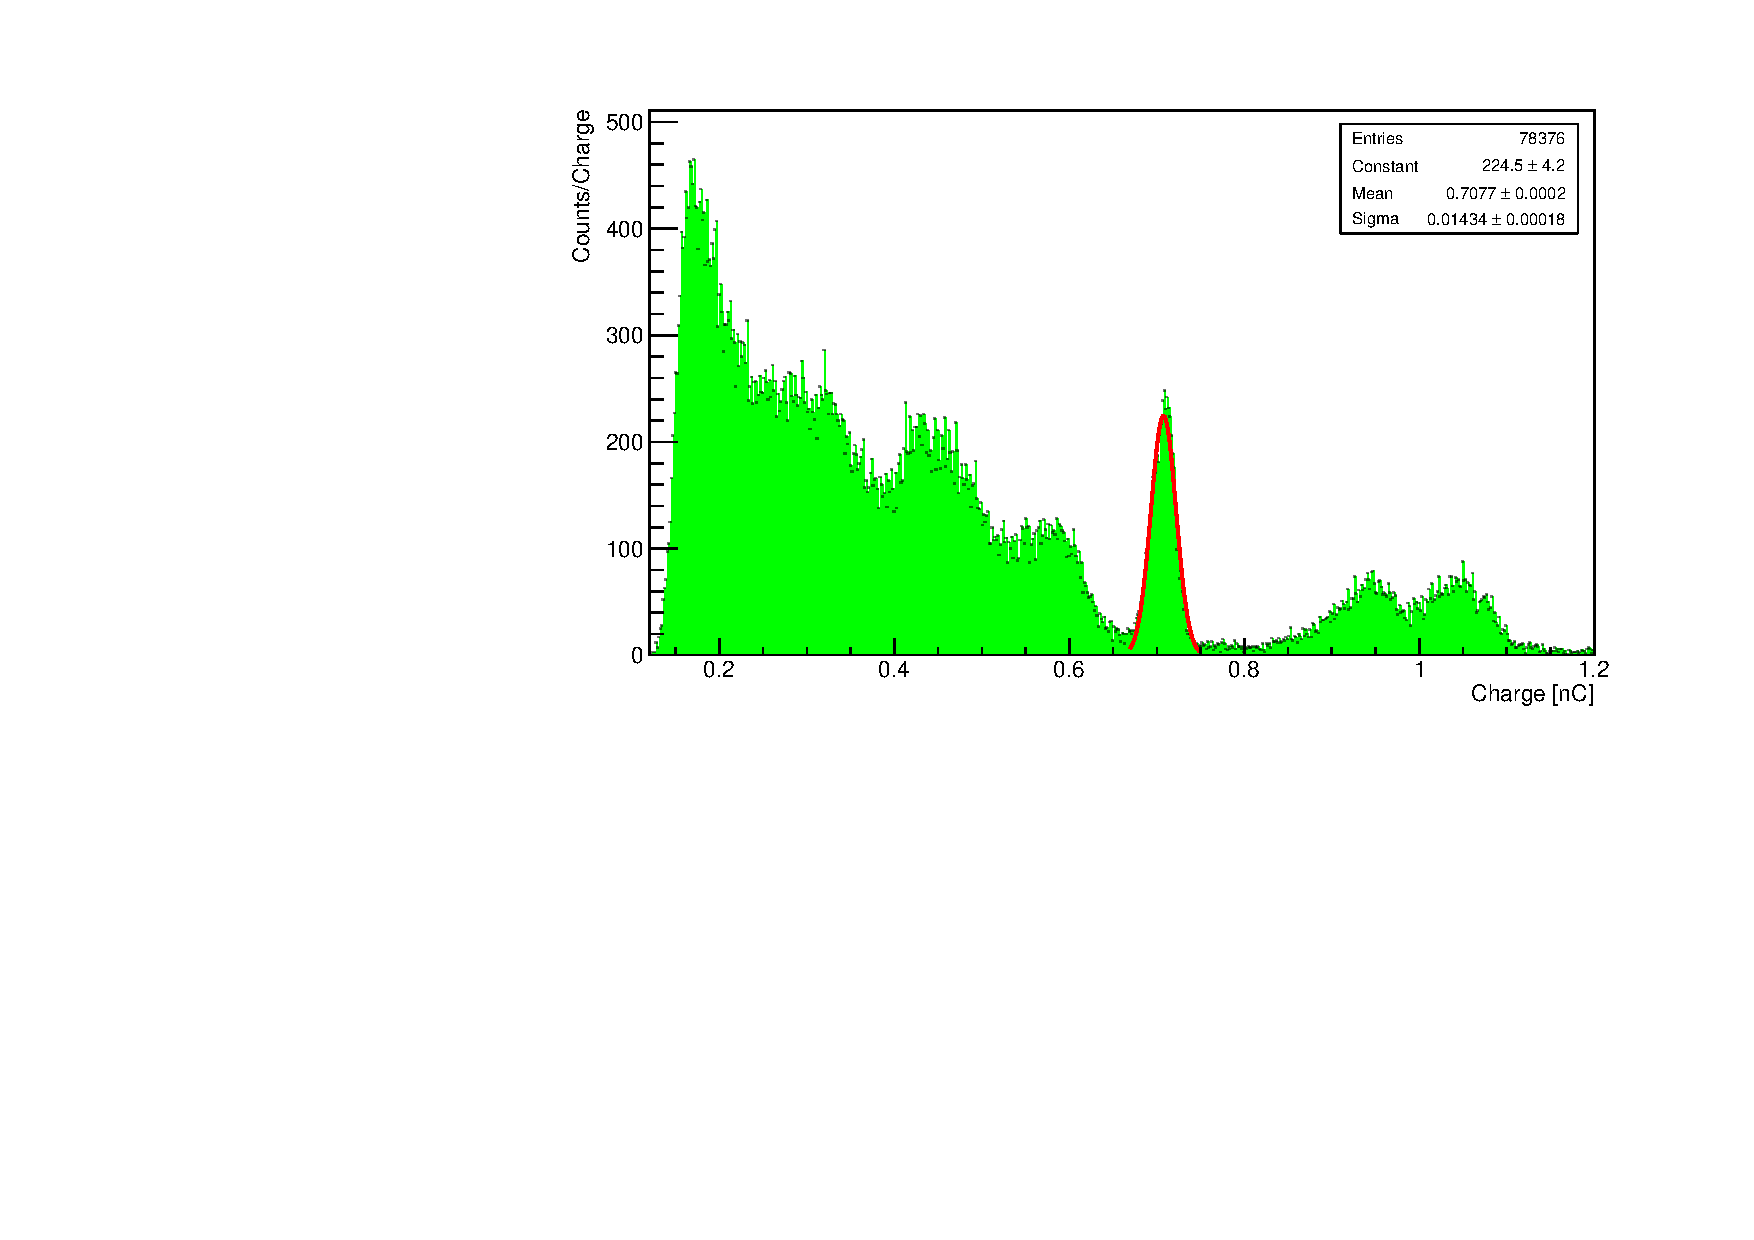
\includegraphics[width=0.7\textwidth]{calibration.pdf}
		\caption{Selfcount spectrum}\label{fig:selfcount}
\end{figure}

\subsection{Multiple hits}
how to handle it?\\
\subsection{Wavelets}
Introuction to Wavelets\\
Discrete Wavelet Transform\\
\subsection{Peak identification}
Chosing Wavelet function for peak identification\\
Heavy ion paper, peak identification\\
\section{Results}
Show multiple pulse in window, and peak identification, cases...
\subsection{Spectrum}
Spectrum for different rates (attenuation filters)\\
Spectrum with multiple pulse, using peak identification and pattern recognition.\\
\subsection{Gamma Flux Rates}
Rate estimation, compare with gain and rate measured with Scaler.




